\documentclass{article}
%%%%%%%%%%%%%%%%%%%%%%%%%%%%%%%%%%%%%%%%%%%%%%%%%%%%%%%%%%%%%%%%%%%%%%%%%%%%%%%
% PREAMBLE
%%%%%%%%%%%%%%%%%%%%%%%%%%%%%%%%%%%%%%%%%%%%%%%%%%%%%%%%%%%%%%%%%%%%%%%%%%%%%%%
\usepackage{mathtools}
\usepackage{algorithm}
\usepackage{algorithmic}
\usepackage{fancyvrb}
\usepackage{booktabs}
\usepackage{rotating}
\usepackage{tikz}
\usepackage{float}
\usepackage{hyperref}
\usepackage{subcaption}
\usetikzlibrary{arrows,decorations.pathmorphing,backgrounds,positioning,fit,matrix}
\newcommand{\DepProps}{\textsc{DepProps}}
\usepackage{titling}
\newcommand{\subtitle}[1]{%
  \posttitle{%
    \par\end{center}
    \begin{center}\large#1\end{center}
    \vskip0.5em}%
}
\begin{document}
% TITLE
\title{DM207 I/O-Efficient Algorithms and Data Structures}
\subtitle{Fall 2015\\Project 1}
% AUTHER
\author{Mikkel Levisen and Jesper Lund}
%DATE
\maketitle
% no page number on first page
\thispagestyle{empty}
\newpage
% TABLE OF CONTENTS
%\tableofcontents
% no page number on table of contents page
\thispagestyle{empty}
\newpage
% restart page number counter
\pagenumbering{arabic} 
%%%%%%%%%%%%%%%%%%%%%%%%%%%%%%%%%%%%%%%%%%%%%%%%%%%%%%%%%%%%%%%%%%%%%%%%%%%%%%%
% DOCUMENT START
%%%%%%%%%%%%%%%%%%%%%%%%%%%%%%%%%%%%%%%%%%%%%%%%%%%%%%%%%%%%%%%%%%%%%%%%%%%%%%%
\section*{Introduction}
The goal of this project is to a feeling of the possible impact of differences 
in memory access patterns on the running time of programs. 

Through this report have the running times been plotted along with an estimate
on of cache and ram sizes.
\\
\\
The machines used in this assignment are the ones from the IMADA terminal room 
and had the following specifications:
\begin{figure}[H]
\centering
\begin{tabular}{lrl}
  Memory type & &size\\ 
  \hline
  L1 	&  	32&kB\\
  L2 	& 	256&kB\\
  L3 	& 	4096&kB\\
  RAM 	& 	3910084& kB
\end{tabular}
\end{figure}
\noindent Since these computers are available to other student at the same time as the 
tests were running it might have effected the results.
\\
\\
Where appropriate we have added dashed lines indicating the estimated cache and 
RAM limits. These guides are only estimates and don't consider other running 
processes. 
\section*{Task 1}
\begin{figure}[H]
    \centering
    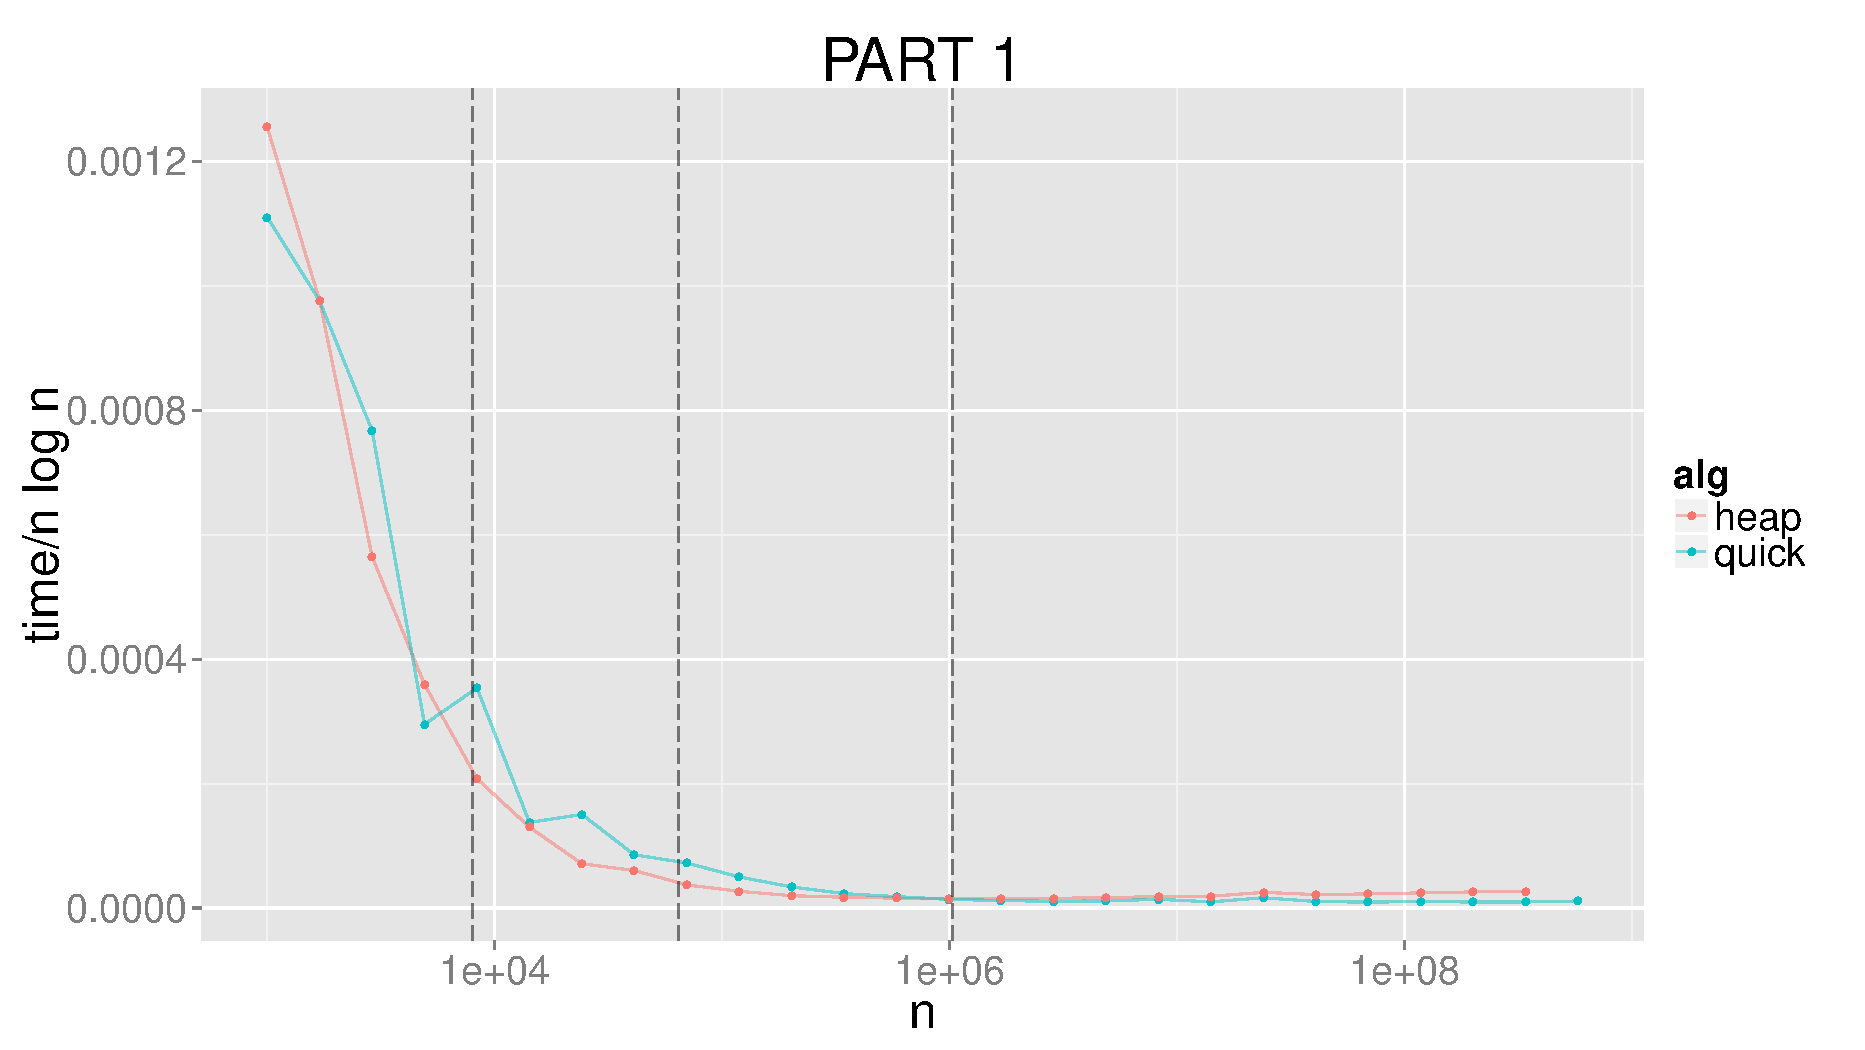
\includegraphics[width=
    \textwidth]{images/part1.pdf}
    \caption{Quicksort vs. Heapsort on arrays of \texttt{int}. 
    \\(\texttt{int}$= 4$ bytes)}
\end{figure}
In figur 1 are arrays of sizes between 1000 and 577011370 containing integers 
sorted with Heapsort and Quicksort. The plot shows the running time of each 
algorithm relative to the expected running time $O(n \log n)$. 

Based on the memory access pattern of the algorithms we are surprised that 
Heapsort seems to outperform Quicksort while handling arrays which fit in cache.

Once the array sizes exceeds the cache limit it clearly show that the spread out
memory access of Heapsort is heavily penalized.
\section*{Task 2}
\begin{figure}[H]
    \centering
    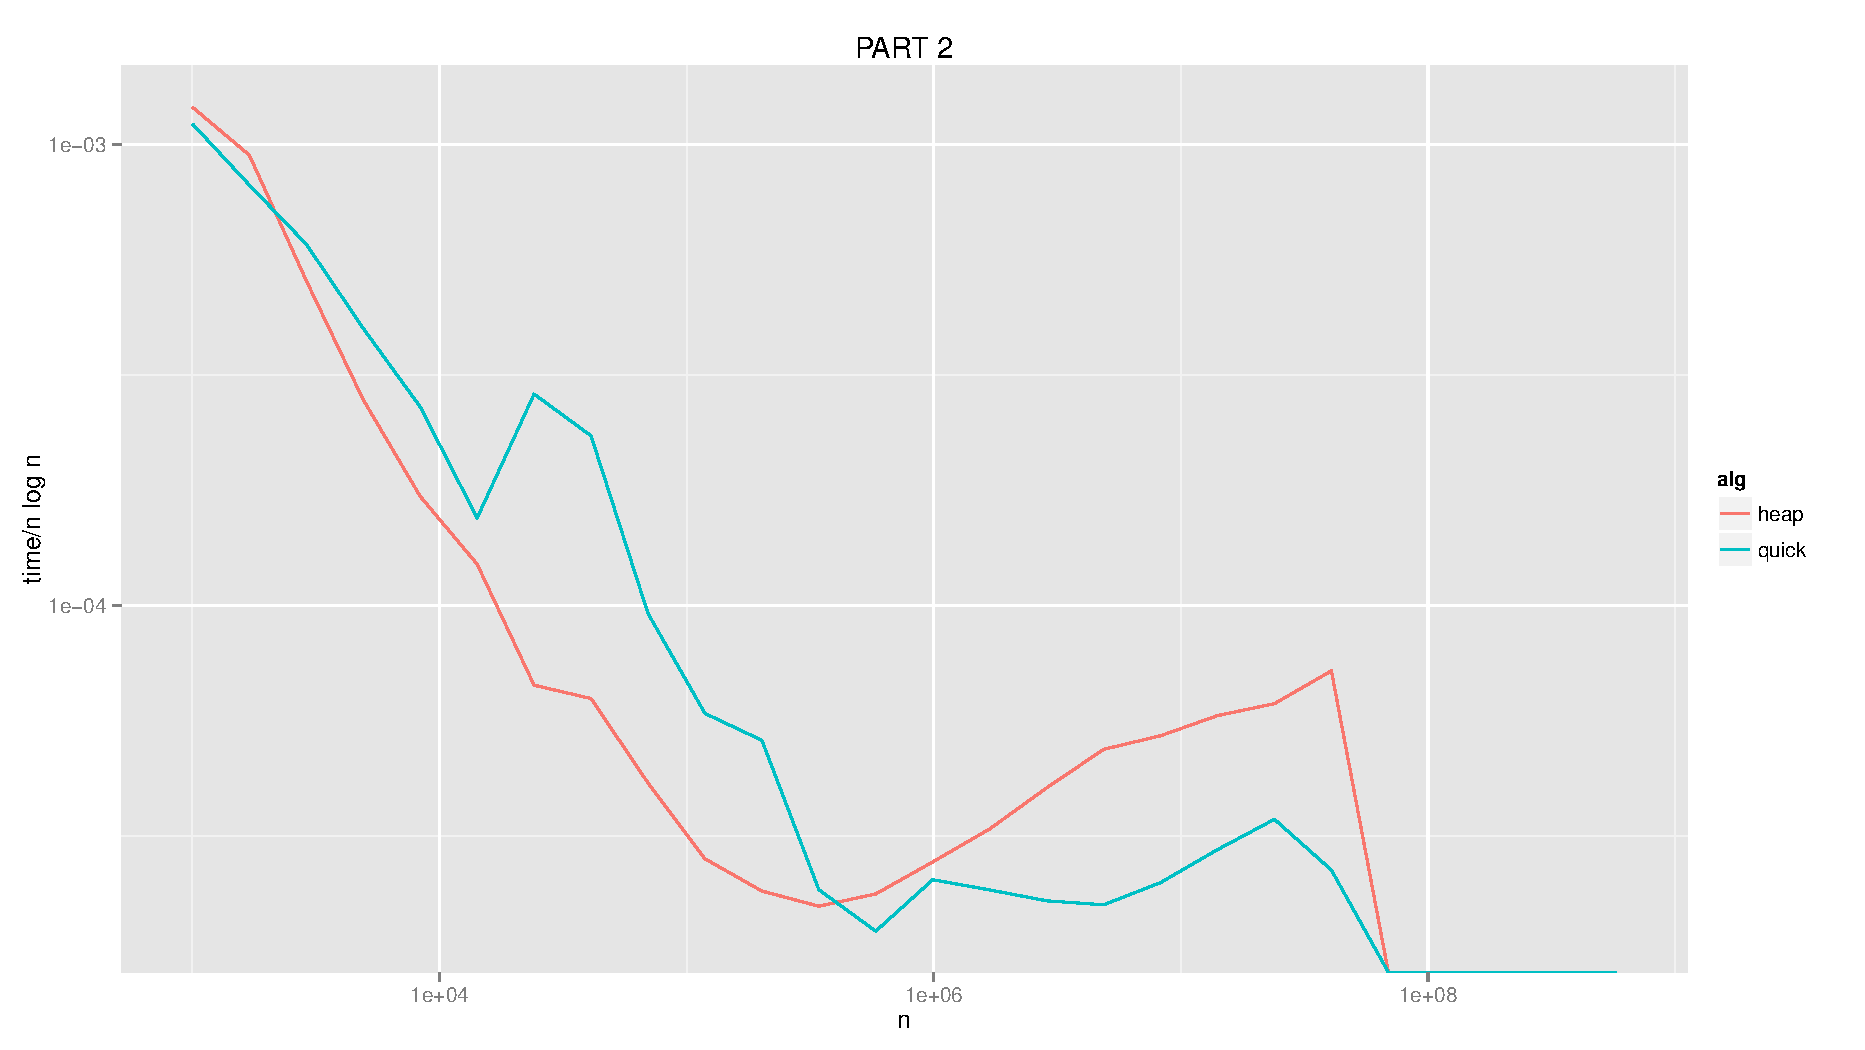
\includegraphics[width=
    \textwidth]{images/part2.pdf}
    \caption{Quicksort vs. Heapsort on arrays of \texttt{Integer}. 
    \\(\texttt{Integer}$= 16$ bytes)}
    \label{fig:awesome_image}
\end{figure}
Because Java uses \textit{pass-by-reference} when dealing with objects will an 
array of objects simply be pointers to memory locations in the heap witch 
removes Quicksort memory access pattern advantage with sequential data.
In figure 2 this is especially visible when the data size reaches L3 cache. In 
RAM Quicksort still has an advantage because it focuses on distinct partitions
of the date rather than the whole set. This leads to a more efficient use of the 
cache.
\section*{Task 3}
\begin{figure}[H]
    \centering
    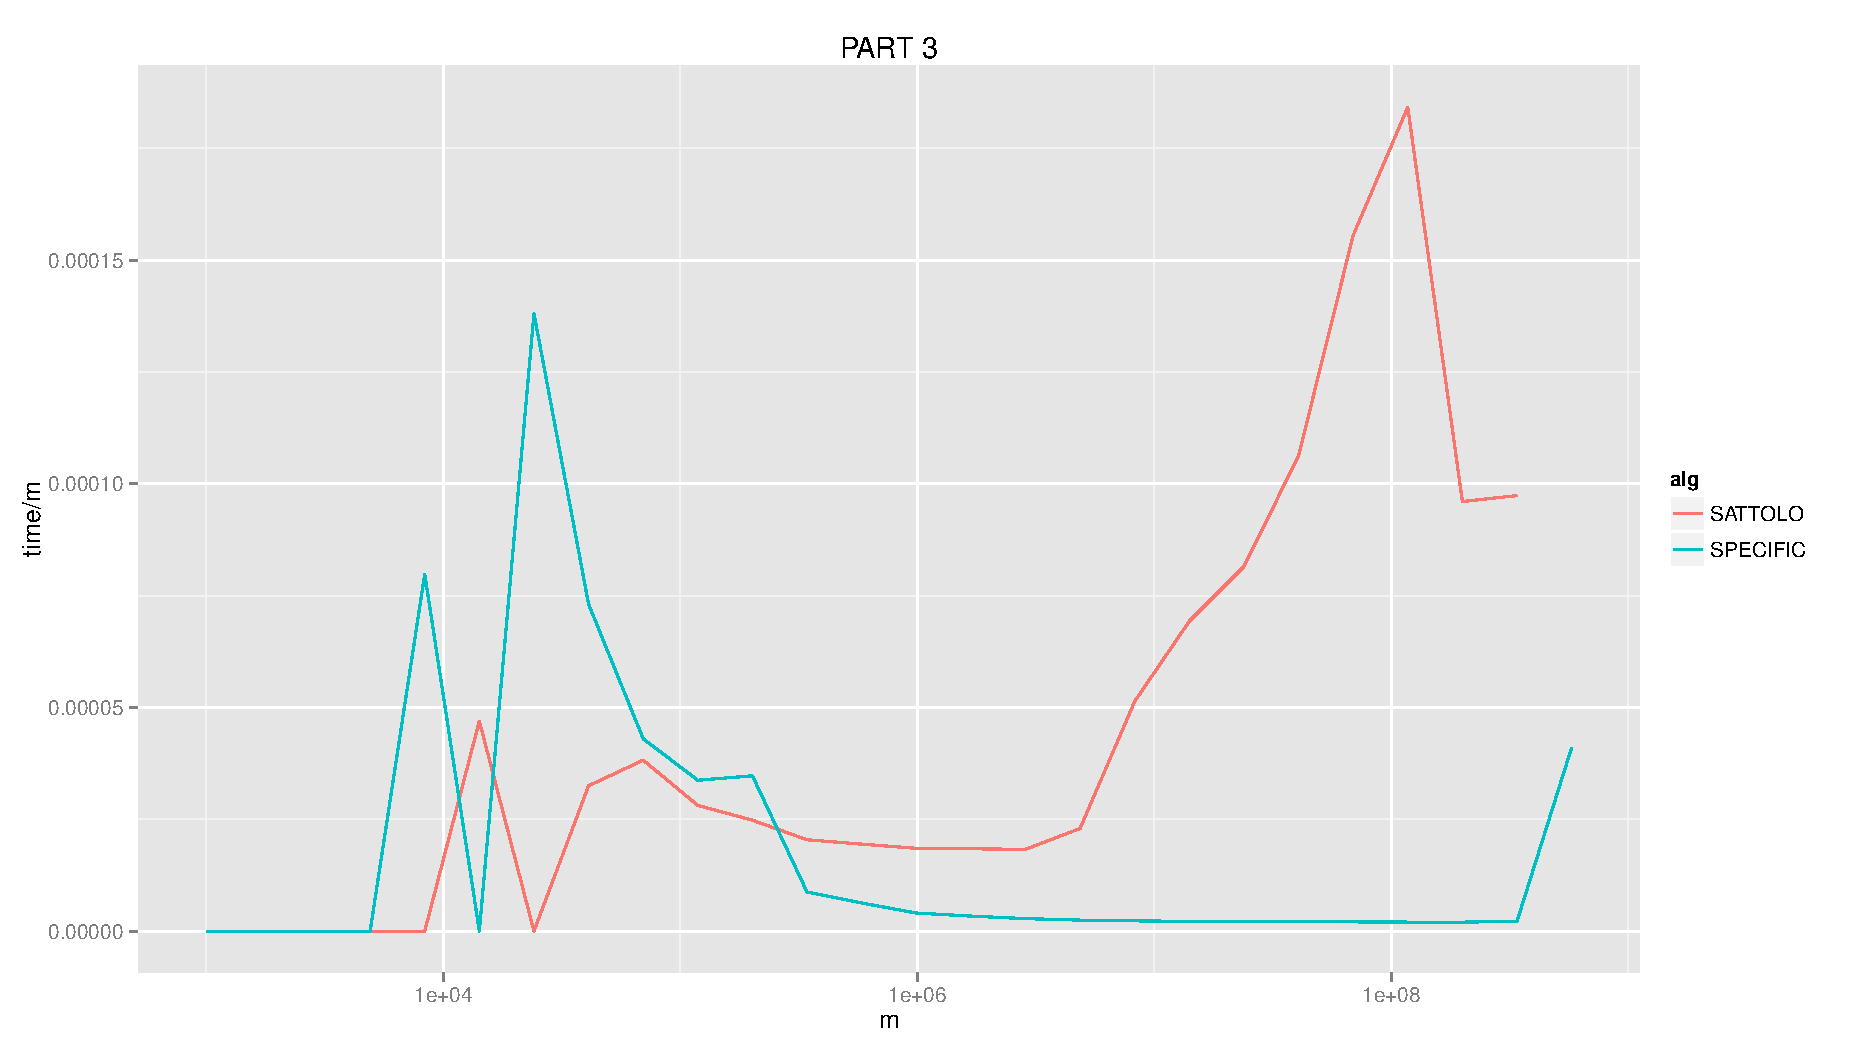
\includegraphics[width=\textwidth]{images/part3.pdf}
    \caption{$n$-cyclic list lookup}
    \label{fig:awesome_image}
\end{figure}
Here we clearly see that SATTOLO performs much worse than a standard $n$-cycle 
because it need to load the same blocks in over and over again where SPECIFIC
only needs to load a block once.
\section*{Task 4}
\begin{figure}[H]
    \centering
    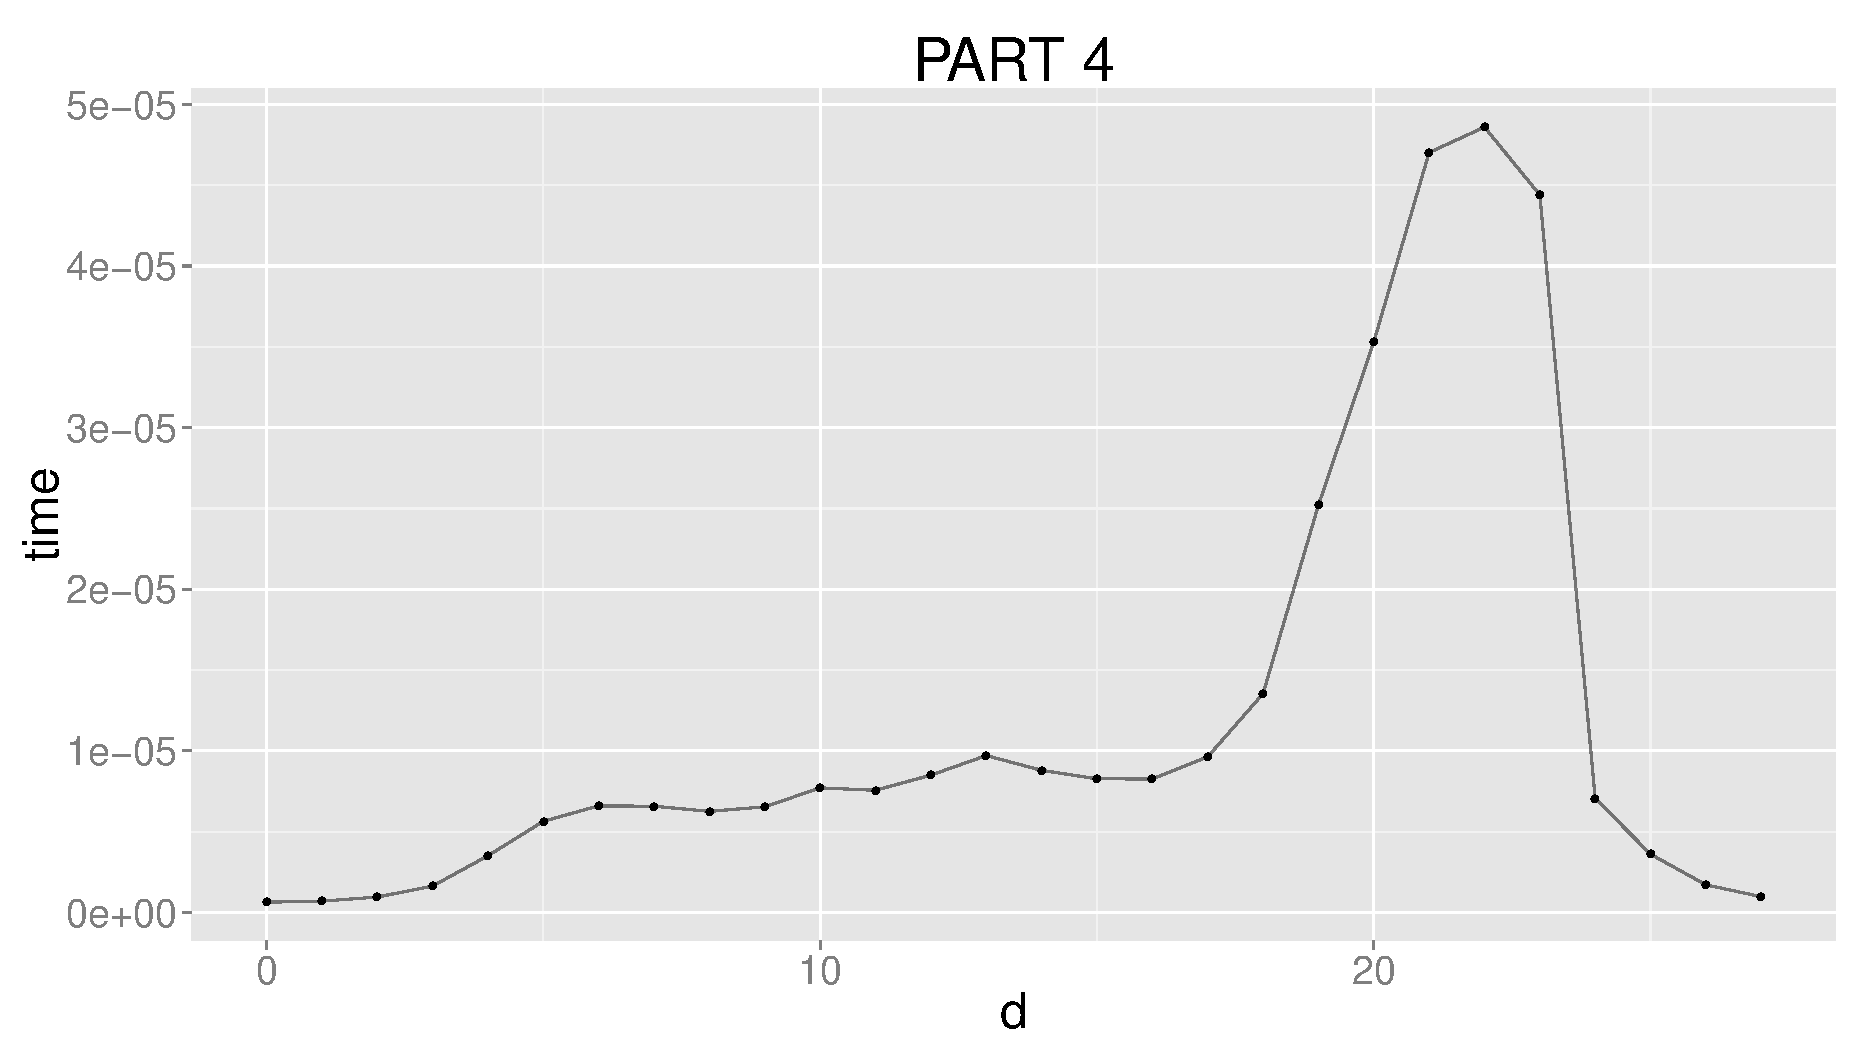
\includegraphics[width=\textwidth]{images/part4.pdf}
    \caption{Random array access}
    \label{fig:awesome_image}
\end{figure}
At each $i$ the number of elements used in each block is halved. This leads to 
doubling the number of block loads. We expected to see an exponential increase 
in running time until reaching a maximum of one block load pr operation. 

Because our cacheline is 64 b and one \texttt{int} is four bytes $d^i$ would 
have to be equal or higher than 16000. 

\section*{Task 5}
\subsection*{5.1}
\begin{figure}[H]
    \centering
    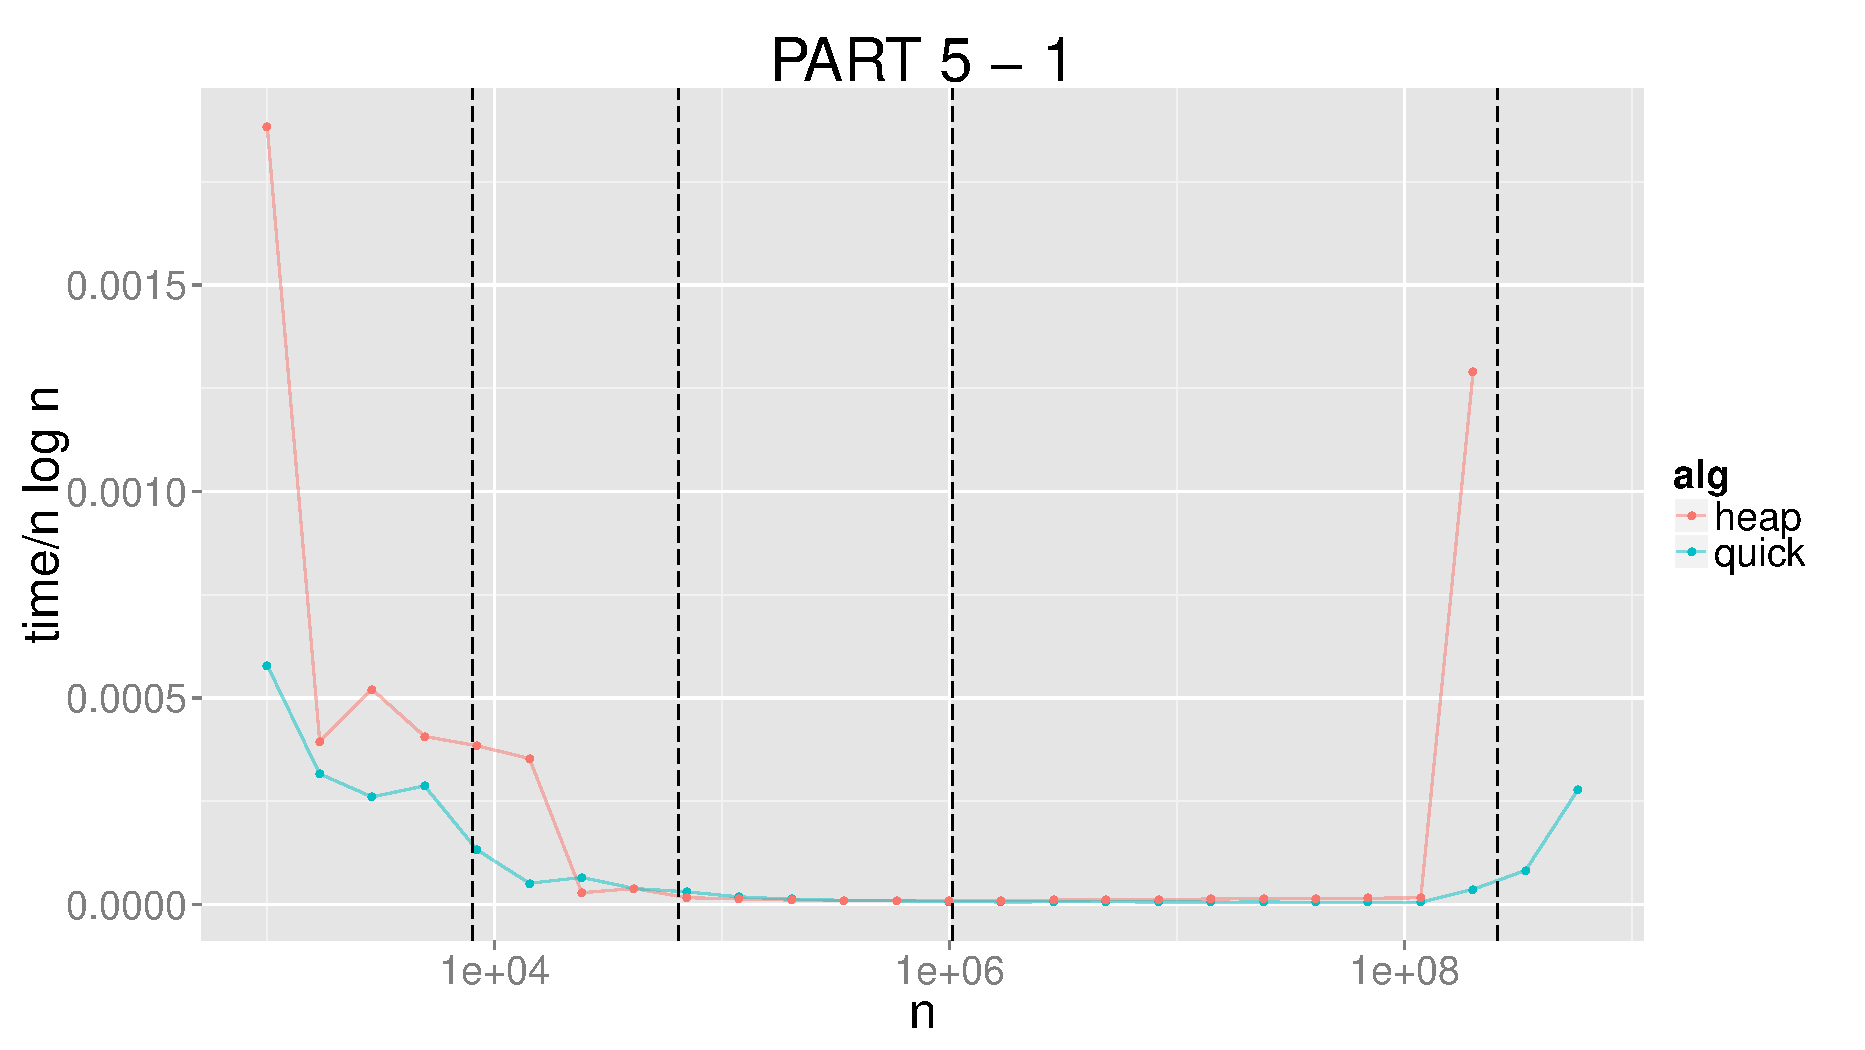
\includegraphics[width=
    \textwidth]{images/part5_1.pdf}
    \caption{Quicksort vs. Heapsort on arrays of \texttt{int}. 
    (\texttt{int}$= 4$ bytes)}
\end{figure}
Here we can clearly see the difference in memory access time when data size 
exceeds cache and RAM. Both Heapsort and Quicksort suffers in speed due to the 
extremely slow load time of the disk. 

Quicksort still outperforms Heapsort since because it deals with data in 
sequential chunks.    
%In figur 1 are arrays of sizes between 1000 and 577011370 containing integers 
%sorted with Heapsort and Quicksort. The plot shows the running time of each 
%algorithm relative to the expected running time $O(n \log n)$. 
%
%Based on the memory access pattern of the algorithms we are surprised that 
%Heapsort seems to outperform Quicksort while handling arrays which fit in cache.
%
%Once the array sizes exceeds the cache limit it clearly show that the spread out
%memory access of Heapsort is heavily penalized.
\subsection*{5.2}
\begin{figure}[H]
    \centering
    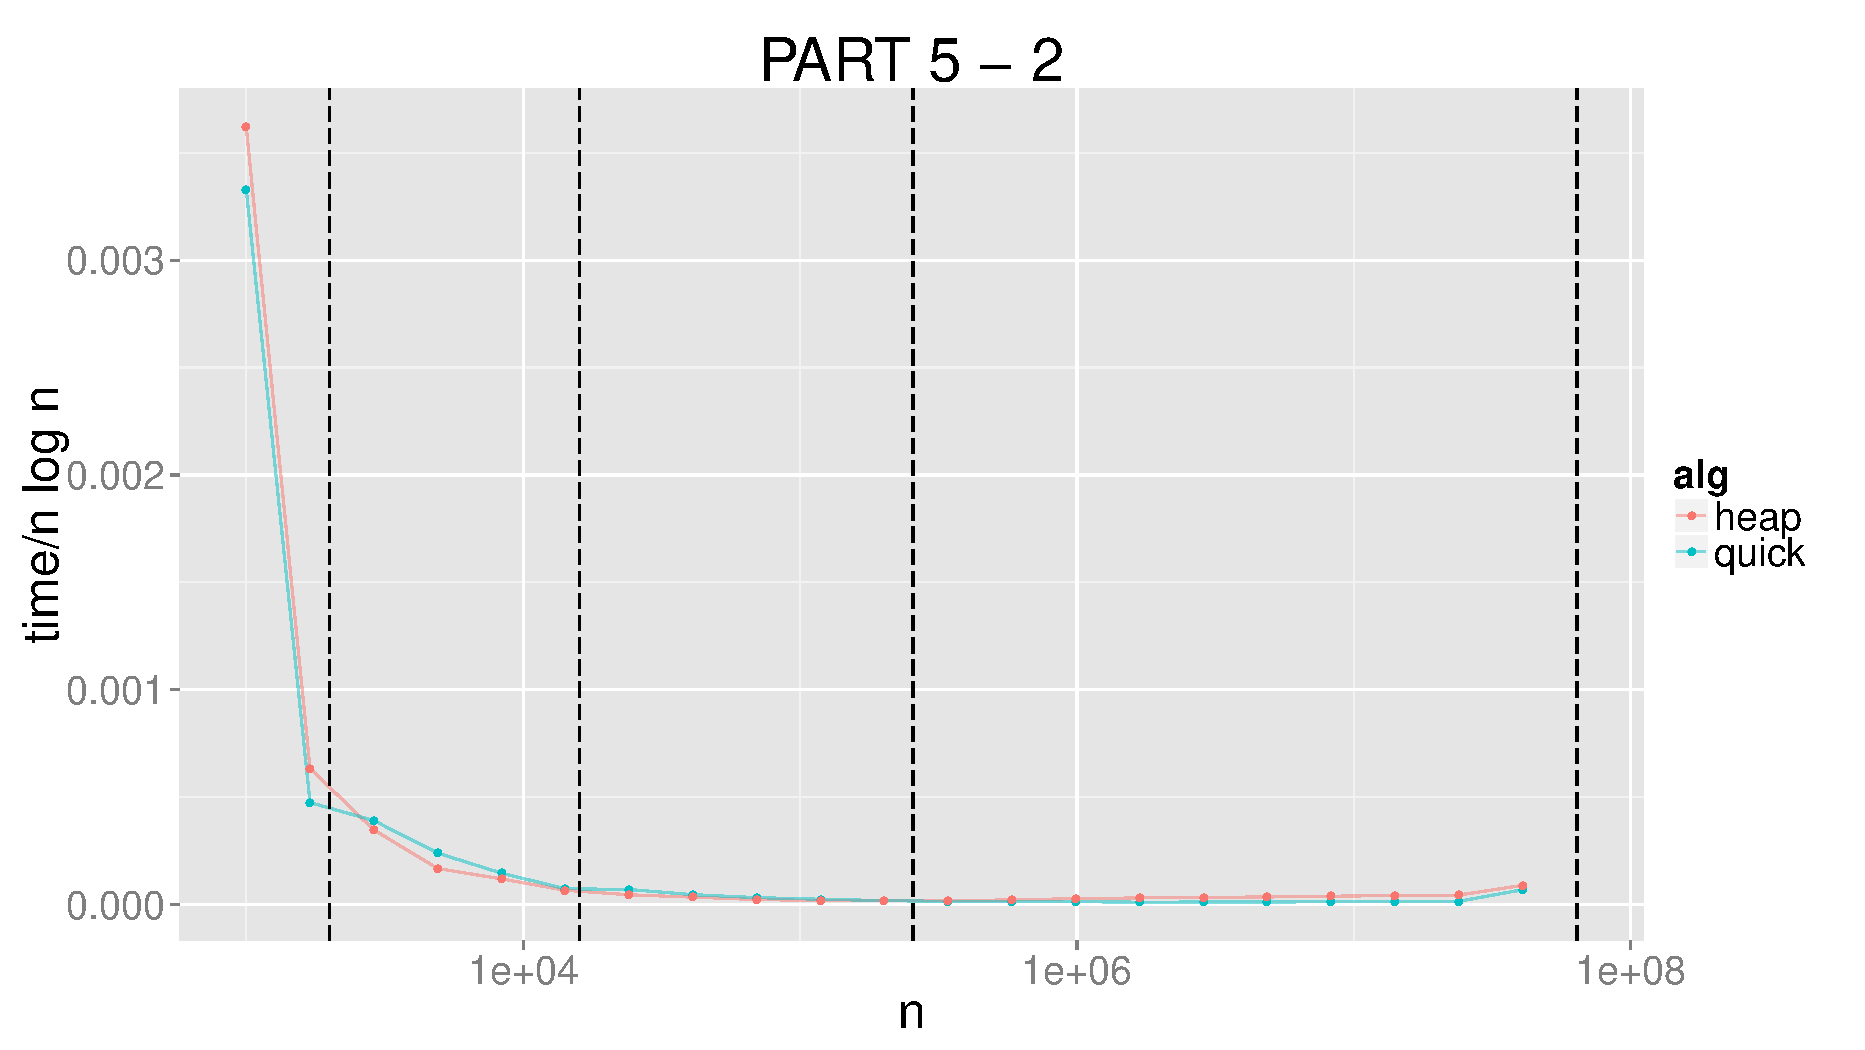
\includegraphics[width=
    \textwidth]{images/part5_2.pdf}
    \caption{Quicksort vs. Heapsort on arrays of \texttt{Integer}. 
    \\(\texttt{Integer}$= 16$ bytes)}
    \label{fig:awesome_image}
\end{figure}
Quicksort still outperforms Heapsort but the effect is less significant because 
of how Java handles objects. Objects outside of ram can now be stored in 
different sectors and would dramatically reduce the efficiency of Quicksort.  

%Because Java uses \textit{pass-by-reference} when dealing with objects will an 
%array of objects simply be pointers to memory locations in the heap witch 
%removes Quicksort memory access pattern advantage with sequential data.
%In figure 2 this is especially visible when the data size reaches L3 cache. In 
%RAM Quicksort still has an advantage because it focuses on distinct partitions
%of the date rather than the whole set. This leads to a more efficient use of the 
%cache.
\subsection*{5.3}
\begin{figure}[H]
    \centering
    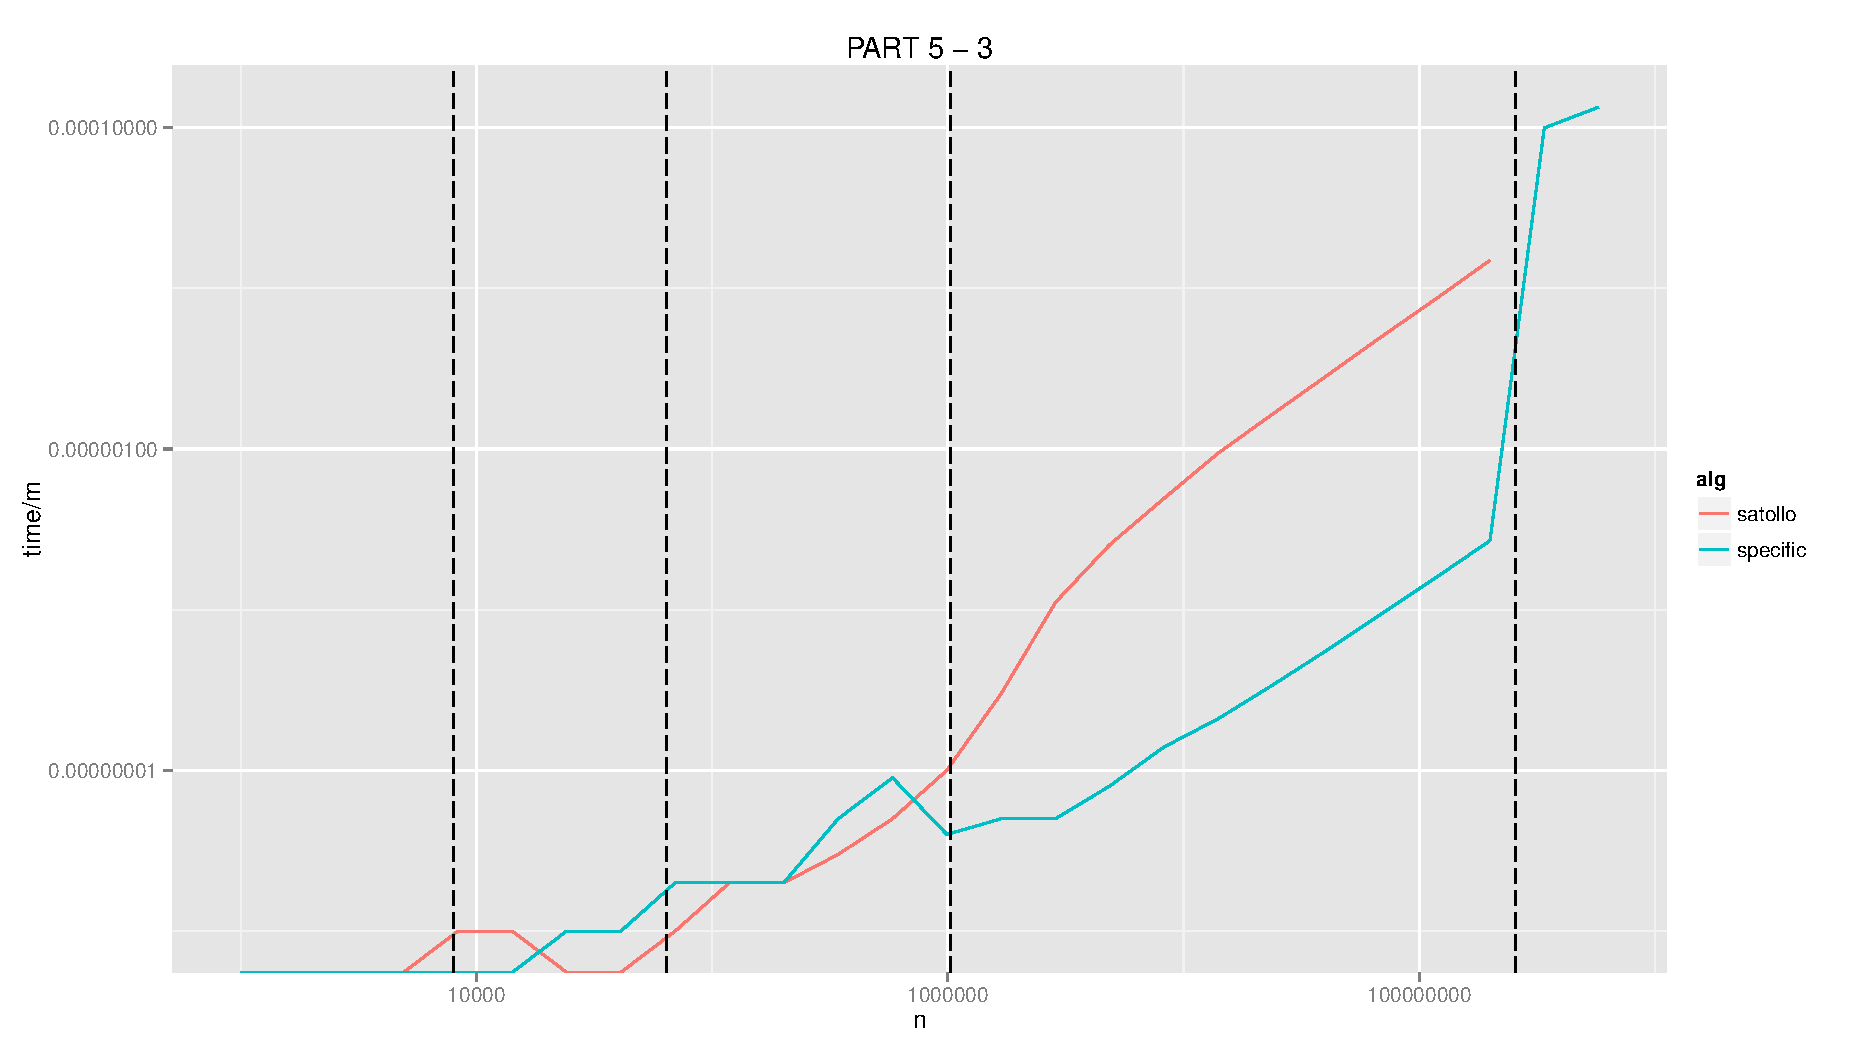
\includegraphics[width=\textwidth]{images/part5_3.pdf}
    \caption{$n$-cyclic list lookup}
    \label{fig:awesome_image}
\end{figure}
Again we see a huge running time penalty from utilizing the disk. Note that 
SATTOLO timed out when it hit the disk. 
\newline
\subsection*{5.4}
\begin{figure}[H]
    \centering
    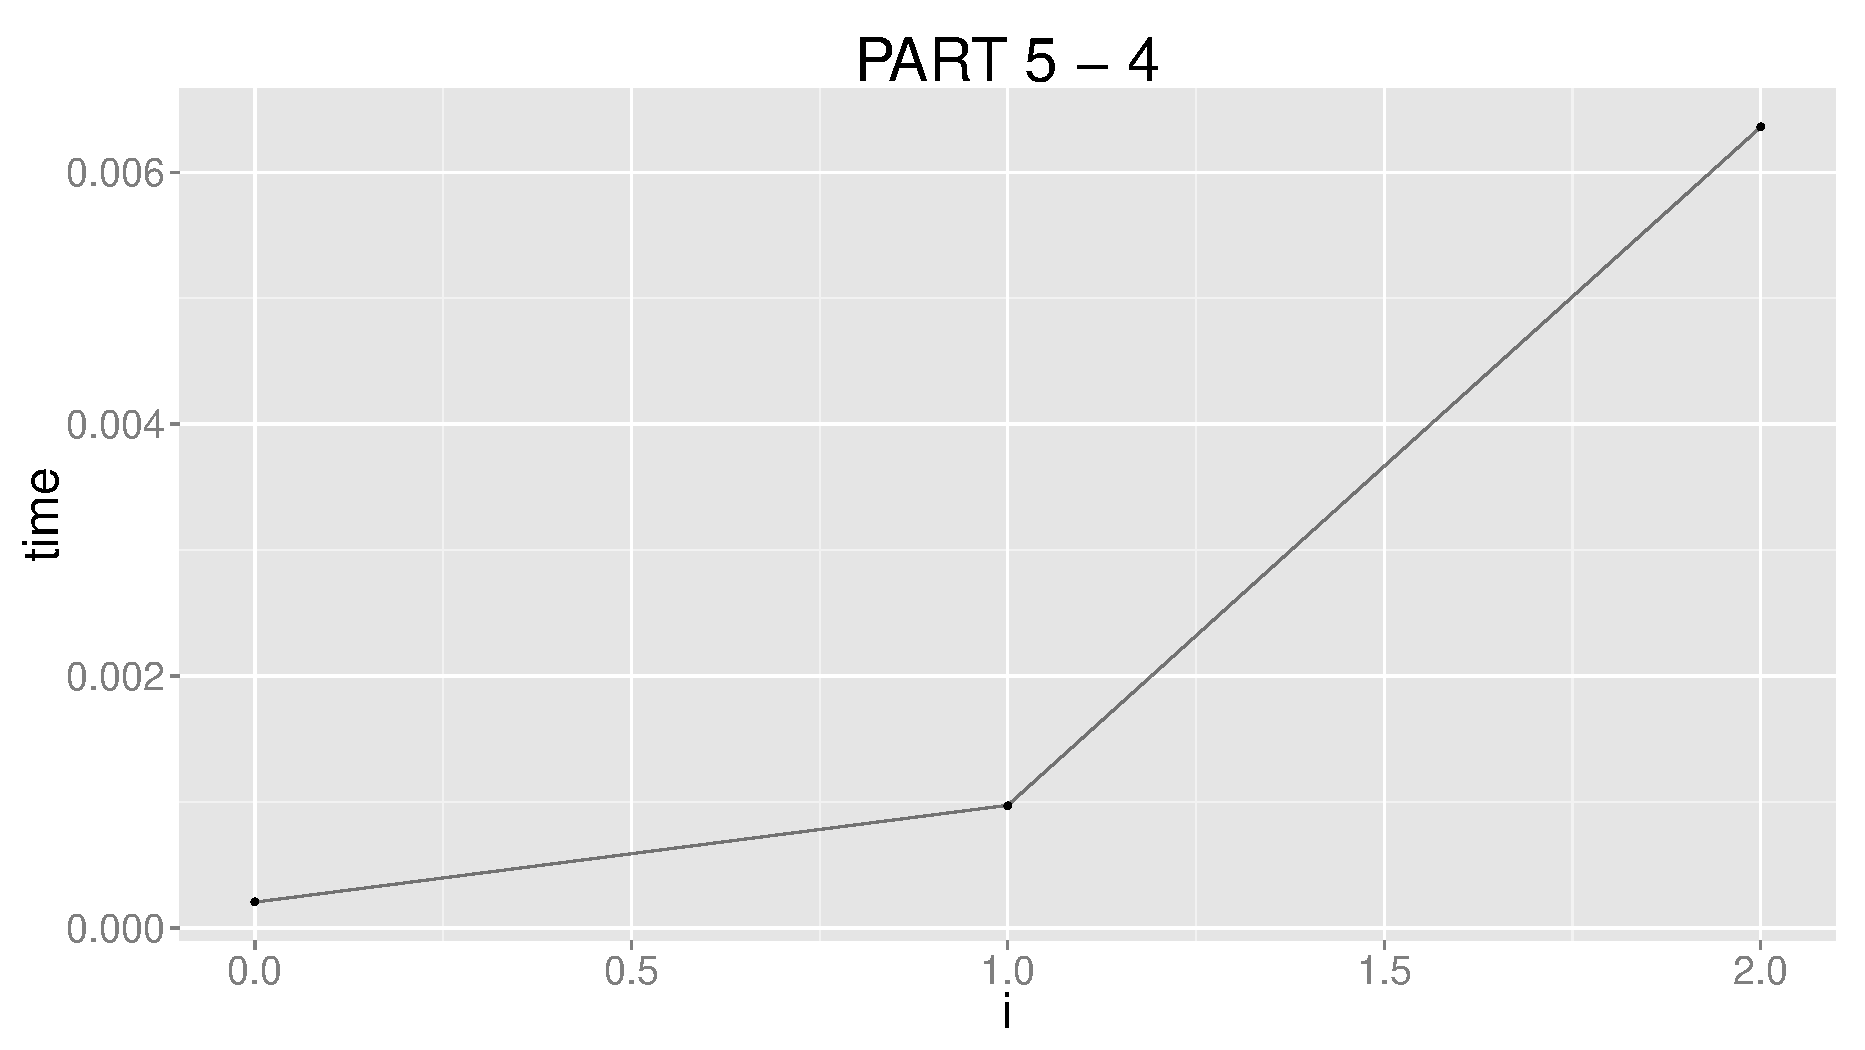
\includegraphics[width=\textwidth]{images/part5_4.pdf}
    \caption{Random array access}
    \label{fig:awesome_image}
\end{figure}
Since the array is larger than the RAM + cache is the 
operation very expensive right from the start, timeing out at $i = 3$. 
%At each $i$ the number of elements used in each block is halved. This leads to 
%doubling the number of block loads. We expected to see an exponential increase 
%in running time until reaching a maximum of one block load pr operation. 
%
%Because our cacheline is 64 kB and one \texttt{int} is four bytes $d^i$ would 
%have to be equal or higher than 16000. 
\end{document}